\documentclass{beamer}
\usepackage{graphicx}
\usepackage{amsmath}


% Set theme and colors
\usecolortheme{default}

% Set font family and other configurations
\usepackage{lmodern}
\renewcommand{\familydefault}{\sfdefault}
\setbeamertemplate{navigation symbols}{}

\title{Mixed Effects Models - Day 3}
\subtitle{Refreshing Linear Models II}
\author{Marieke Wesselkamp \\ Department of Biometry and Environmental Systems Analysis \\ Albert-Ludwigs-University of Freiburg (Germany)}
\date{February 2023}

\begin{document}

\begin{frame}
  \titlepage
\end{frame}

\begin{frame}{Recap Yesterday}
  \textbf{The relationship between a \textit{continuous} predictor variable and a continuous response variable...}
  
  \begin{figure}[h]
    \centering
    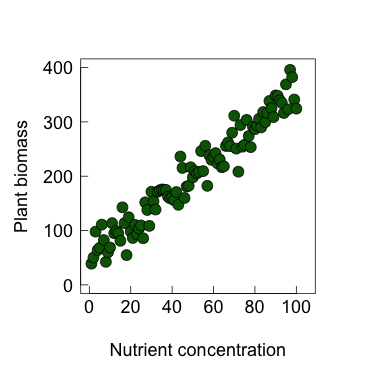
\includegraphics[width=0.5\textwidth]{lectures/day_3_LM_refresh_II/figures/unnamed-chunk-2-1.png} 
    \caption{Scatterplot of nutrient concentration vs. plant biomass.}
  \end{figure}
\end{frame}

\begin{frame}
  \frametitle{}
  \textbf{...can be described by this \textit{model}:}
  
  \begin{equation*}
  y = \beta_0 + \beta_1 \cdot x + \epsilon
  \end{equation*}
  
  \begin{figure}[h]
    \centering
    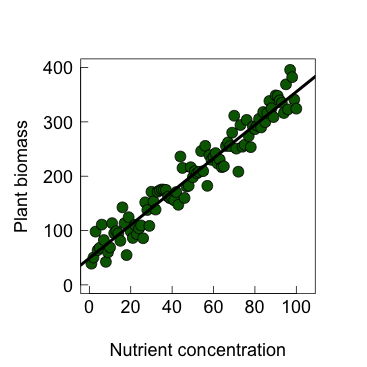
\includegraphics[width=0.5\textwidth]{lectures/day_3_LM_refresh_II/figures/unnamed-chunk-3-1.png} 
    \caption{Linear model fit to the data.}
  \end{figure}
\end{frame}

\begin{frame}
  \frametitle{Matrix Notation}
  \textbf{In matrix notation:}
  
  \begin{equation*}
  \mathbf{y} = \mathbf{X} \cdot \mathbf{\beta} + \mathbf{e}, \quad \epsilon_{iid} \sim \mathcal{N}(0, \sigma^2_{\epsilon} \cdot \mathbf{I})
  \end{equation*}
  where $\mathbf{y}$ are the measured response values, $\mathbf{X}$ is the Design matrix, $\mathbf{\beta}$ is a vector of model parameters, $\mathbf{e}$ is a vector of the errors $\epsilon$, and $\sigma^2_{\epsilon} \cdot \mathbf{I}$ is the variance-covariance matrix of the errors.
\end{frame}

\begin{frame}
  \frametitle{Variance-Covariance Matrix of the Errors}
  \textbf{The variance-covariance matrix of the \textit{errors}...}

  with $\epsilon_{iid} \sim \mathcal{N}(0, \sigma^2_{\epsilon} \cdot \mathbf{I})$:
  
  \begin{equation*}
  \scriptsize{\left( \begin{array}{ccccc} 1.52 & 0 & 0 & 0 & 0 \\ 0 & 1.52 & 0 & 0 & 0 \\ 0 & 0 & 1.52 & 0 & 0 \\ 0 & 0 & 0 & 1.52 & 0 \\ 0 & 0 & 0 & 0 & 1.52 \end{array}\right)}
  \end{equation*}

  \begin{itemize}
    \item \textbf{Note:} The variances are on the diagonals, and the covariances are on the off-diagonals.
  \end{itemize}
\end{frame}

\begin{frame}
  \frametitle{}
  \textbf{...is not the variance-covariance matrix of the \textit{parameters}.}
  
  \begin{itemize}
    \item The variance-covariance matrix of parameters is different and involves correlations among the model parameters.
  \end{itemize}
\end{frame}

\begin{frame}
  \frametitle{}
  \begin{center}
    \huge\textbf{\textcolor{purple}{Categorical predictors}}
  \end{center}
\end{frame}

\begin{frame}
  \frametitle{}
  \textbf{The design matrix for a continuous predictor:}

  \begin{equation*}
  \mathbf{x} = \left( \begin{array}{cc} 1 & x_{1} \\ 1 & x_{2} \\ . & . \\ . & . \\ . & . \\ 1 & x_{n-1} \\ 1 & x_n \end{array}\right)
  \end{equation*}

  with 1's for the intercept and a column with the actual x-values.
\end{frame}

\begin{frame}
  \frametitle{}
  \textbf{What if there are only two values of a predictor with several measurements of the response at these values?*}

  \begin{itemize}
    \item \textbf{Note:} This is \textit{NOT} grouping as long as the measurements taken at the same predictor value are from \textit{different} units.
  \end{itemize}
  
  \begin{figure}[h]
    \centering
    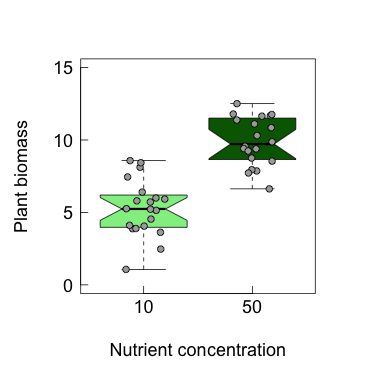
\includegraphics[width=0.5\textwidth]{lectures/day_3_LM_refresh_II/figures/unnamed-chunk-8-1.png} 
    \caption{Boxplot of response by nutrient concentration.}
  \end{figure}
\end{frame}

\begin{frame}
  \frametitle{}
  \textbf{The question is now usually not how the response increases with the predictor, but what the \textit{difference} in the response between the low and high values of the predictor is.}
  
  \begin{figure}[h]
    \centering
    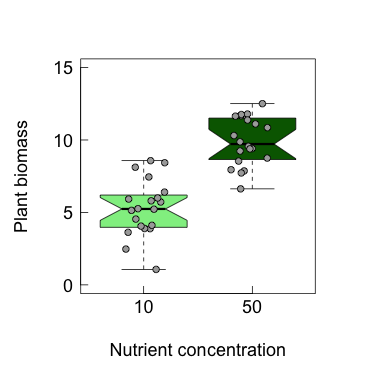
\includegraphics[width=0.5\textwidth]{lectures/day_3_LM_refresh_II/figures/unnamed-chunk-9-1.png} 
    \caption{Difference in response by nutrient concentration.}
  \end{figure}
\end{frame}

\begin{frame}
  \frametitle{}
  \textbf{The matrix notation is identical...}

  \begin{equation*}
  \mathbf{y} = \mathbf{X} \cdot \mathbf{b} + \mathbf{e}, \quad \epsilon \sim \mathcal{N}(0, \sigma^2_{\epsilon} \cdot \mathbf{I})
  \end{equation*}
\end{frame}

\begin{frame}
  \frametitle{}
  \textbf{...but the design matrix for a \textit{categorical} predictor looks different:}

  \begin{equation*}
  \tiny {\mathbf{x} = \left( \begin{array}{cc} 1 & 0 \\ 1 & 0 \\ 1 & 0 \\ . & . \\ . & . \\ 1 & 1 \\ 1 & 1 \\ 1 & 1 \end{array}\right) }
  \end{equation*}
  
  The categorical (here: binary) variable is encoded as 0 and 1, regardless of its content. This is a \textit{dummy variable} that takes 0 for the first and 1 for the second treatment level.
\end{frame}

\begin{frame}
  \frametitle{}
  \textbf{This changes the interpretation of our linear model parameters:}

  \begin{equation*}
  y = \beta_0 + \beta_1 \cdot x + \epsilon
  \end{equation*}
  
  What happens when $x$ is 0?
  
  \begin{equation*}
  y = \beta_0 + \beta_1 \cdot 0 + \epsilon = \beta_0 + \epsilon
  \end{equation*}
  
  $\beta_0$ now represents the mean of the first treatment, and $\beta_1$ the difference of the second treatment to that mean.
  
  \begin{figure}[h]
    \centering
    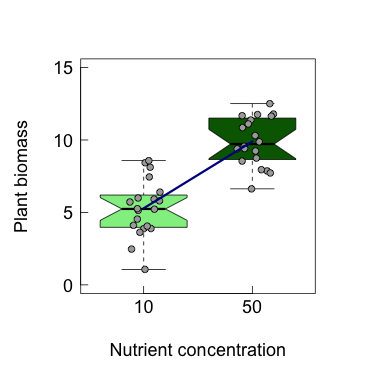
\includegraphics[width=0.5\textwidth]{lectures/day_3_LM_refresh_II/figures/unnamed-chunk-10-1.png} 
    \caption{Interpretation of model parameters.}
  \end{figure}
\end{frame}

\begin{frame}
  \frametitle{}
  \textbf{Accordingly, multiple levels are encoded into multiple dummy variables.}
  
  \begin{figure}[h]
    \centering
    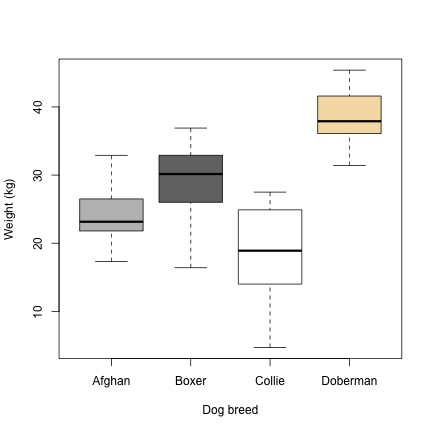
\includegraphics[width=0.6\textwidth]{lectures/day_3_LM_refresh_II/figures/unnamed-chunk-12-1.png} 
    \caption{Boxplot of dog weights by breed.}
  \end{figure}
\end{frame}

\begin{frame}
  \frametitle{}
  \textbf{With k categories, there are k-1 dummy variables, each representing a unique category.}
  
  \begin{equation*}
  \tiny {\mathbf{x} = \left( \begin{array}{cccc} 1 & 0 & 0 & 0 \\ 1 & 0 & 0 & 0 \\ 1 & 1 & 0 & 0 \\ 1 & 1 & 0 & 0 \\ 1 & 0 & 1 & 0 \\ 1 & 0 & 1 & 0 \\ 1 & 0 & 0 & 1\\ 1 & 0 & 0 & 1 \end{array}\right) }
  \end{equation*}

  with the first column of 1's for the first mean and the other columns of 0's and 1's for the \textit{differences} to that baseline.
\end{frame}

\begin{frame}
  \frametitle{}
  \begin{figure}[h]
    \centering
    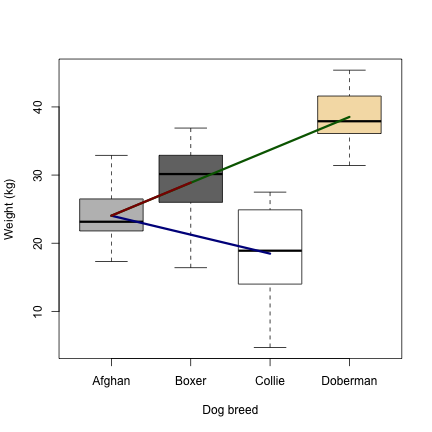
\includegraphics[width=0.6\textwidth]{lectures/day_3_LM_refresh_II/figures/unnamed-chunk-13-1.png} 
    \caption{Differences between breeds.}
  \end{figure}
\end{frame}

\begin{frame}
  \frametitle{}
  \begin{center}
    \huge\textbf{\textcolor{purple}{Analysis of variance with a binary predictor}}
  \end{center}
\end{frame}

\begin{frame}
  \frametitle{ANOVA Table}

  \resizebox{\linewidth}{!}{
  \begin{tabular}{lccccc}
    Source & SS & df & MS & F & p \\
    \hline
    Treatment & SS$_{Treat}$ & k$_{Treat}$ - 1 & SS$_{Treat}$ / df$_{Treat}$ & MS$_{Treat}$ / MS$_{Res}$ \\
    Residual & SS$_{Res}$  & N - k & SS$_{Res}$ / df$_{Res}$ \\
    Total & SS$_{Total}$ & N - 1 \\
  \end{tabular}}
  
  \vspace{1cm}
  \begin{equation*}
  Variance_{total} = Variance_{treatment} + Variance_{residual}
  \end{equation*}
\end{frame}

\begin{frame}
  \frametitle{}
  \textbf{aov()} strongly focuses on hypothesis tests, less on parameter estimation.
\end{frame}

\begin{frame}
  \frametitle{}
  \textbf{lm()} and \textbf{aov()} give the same results but in different formats.
\end{frame}

\begin{frame}{}
  \begin{center}
    \huge\textbf{\textcolor{purple}{Multiple predictors}}
  \end{center}
\end{frame}

\begin{frame}{Multivariate Regression}
  As soon as we have more than two predictors:
  
  \begin{itemize}
      \item \texttt{lm(y \textasciitilde{} x.1 + x.2 + ... + x.n,...)}
  \end{itemize}
  
  The \textbf{deterministic part} requires \textit{at least} n + 1 coefficients:
  
  \begin{equation*}
    \mathbf{y} = \beta_0 + \beta_1 \cdot x_1 + \beta_2 \cdot x_2 + ... + \beta_n \cdot x_n 
  \end{equation*}
\end{frame}

\begin{frame}
  \frametitle{}
  Predictors can be only categorical, only continuous, or a mixture of both.
  \vspace{0.5cm}
  \begin{table}[h]
    \centering
    \begin{tabular}{ccc}
      \hline
      $\mathbf{y}$ & $x_1$ & $x_2$ \\
      \hline
      3.32 & 1.0 & control \\
      4.32 & 2.3 & control \\
      2.09 & 4.2 & control \\
      . & . & . \\
      . & . & . \\
      2.12 & 2.0 & treatment \\
      4.02 & 4.1 & treatment \\
      8.12 & 5.4 & treatment \\
      \hline
    \end{tabular}
  \end{table}
\end{frame}

\begin{frame}
  \frametitle{}
  Exemplary design matrix for one continuous and one binary predictor:
  
  \begin{equation*}
  \mathbf{x} = \left( \begin{array}{ccc} 1 & x_{1} & 0 \\ 1 & x_{2} & 0 \\ 1 & x_{3} & 0 \\ . & . & . \\ . & . & . \\ 1 & x_{n-2} & 1 \\ 1 & x_{n-1} & 1 \\ 1 & x_n & 1 \end{array}\right)
  \end{equation*}
\end{frame}

\begin{frame}
  \frametitle{}
  \textbf{Why not simply use two univariate models, one per predictor?}
  
  \begin{itemize}
    \item \texttt{lung capacity} \textit{may} depend on \texttt{smoking} and \texttt{age}.
  \end{itemize}
\end{frame}

\begin{frame}
  \frametitle{}
\textbf{First univariate model: smoking increases lung capacity by nearly a liter}
  
  \begin{figure}[h]
    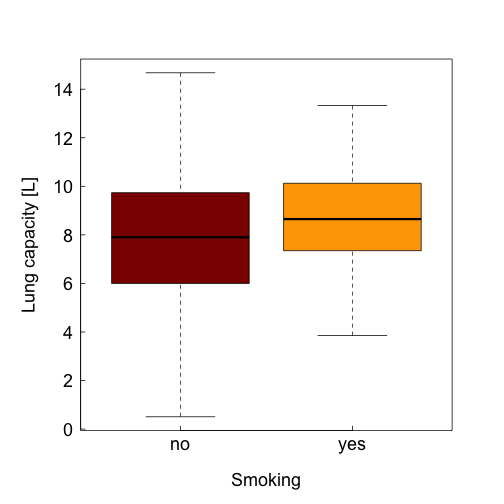
\includegraphics[width=0.6\textwidth]{lectures/day_3_LM_refresh_II/figures/unnamed-chunk-21-1.png} 
    \caption{Boxplot of lung capacity by smoking status.}
  \end{figure}
\end{frame}

\begin{frame}
  \frametitle{}
\textbf{Second univariate model: aging increases lung capacity by half a liter every year (a body growth effect)}
  
  \begin{figure}[h]
    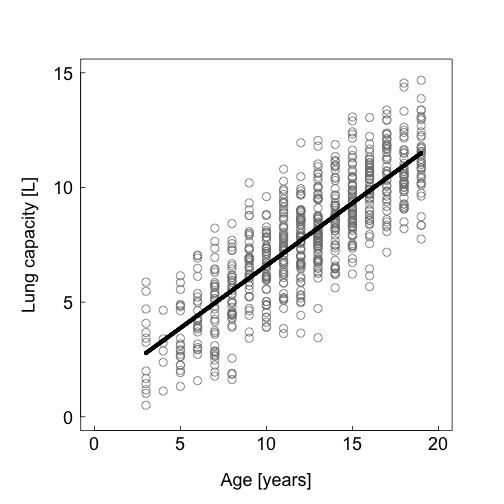
\includegraphics[width=0.6\textwidth]{lectures/day_3_LM_refresh_II/figures/unnamed-chunk-23-1.png} 
    \caption{Boxplot of lung capacity by age in years.}
  \end{figure}
\end{frame}

\begin{frame}
  \frametitle{}
\textbf{Smoking and Age are correlated = confounded\footnote{biserial correlations are between a continuous and a categorical random variable}.\\ Children (hopefully) don't smoke but have small lungs.}
  
  \begin{figure}[h]
    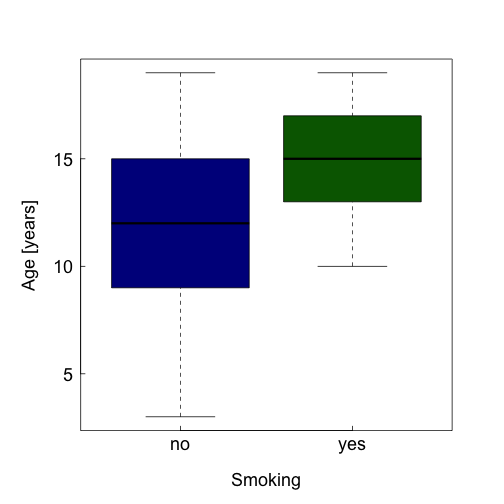
\includegraphics[width=0.6\textwidth]{lectures/day_3_LM_refresh_II/figures/unnamed-chunk-25-1.png} 
    \caption{Boxplot of lung capacity by smoking status.}
  \end{figure}
\end{frame}

\begin{frame}
  \frametitle{}
  \textbf{Now a multivariate model:}
  
  \begin{itemize}
    \item \texttt{m <- glm(LungCap \textasciitilde{} Age + Smoke, data = lung)}
  \end{itemize}
\vspace{0.5cm}

\begin{tabular}{cl}  
    \begin{tabular}{c}
        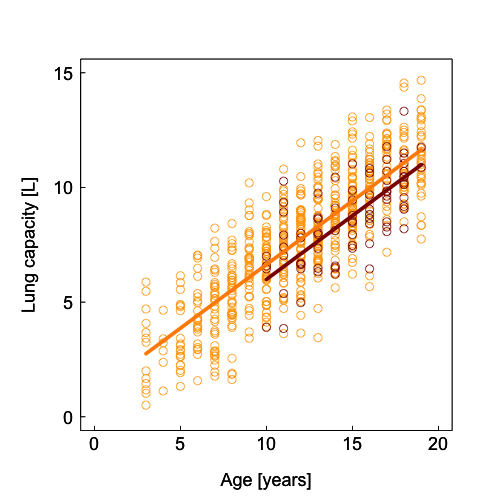
\includegraphics[width=0.4\textwidth]{lectures/day_3_LM_refresh_II/figures/unnamed-chunk-28-1.png}
    \end{tabular}
    & 
    \begin{tabular}{l}
        \parbox{0.5\linewidth}{
        \textbf{Indeed, smoking decreases lung capacity by 0.65 liter.}}
    \end{tabular}  \\
\end{tabular}
\end{frame}

\begin{frame}
\frametitle{Predictions}
\begin{tabular}{cl}
    \begin{tabular}{c}
        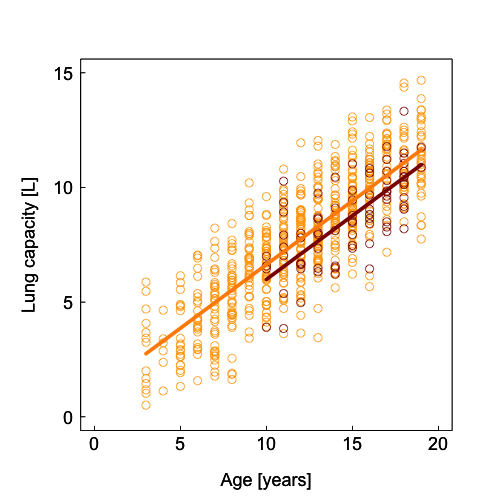
\includegraphics[width=0.4\textwidth]{lectures/day_3_LM_refresh_II/figures/unnamed-chunk-28-1.png}
    \end{tabular}
    &
    \begin{tabular}{l}
        \parbox{0.5\linewidth}{
          A 15-year-old \textbf{smoker} has an expected lung capacity of:
          \begin{equation*}
          1.09 + 0.56 \cdot 15 - 1 \cdot 0.65 = 8.84 \text{ liters.}
          \end{equation*}
          A 15-year-old \textbf{non-smoker} has an expected lung capacity of:
          \begin{equation*}
          1.09 + 0.56 \cdot 15 - 0 \cdot 0.65 = 9.49 \text{ liters.}
          \end{equation*}
          }
    \end{tabular}
\end{tabular}
\end{frame}

\begin{frame}
  \frametitle{Reasons for Multivariate Regression}
  \begin{itemize}
    \item Multiple causation
    \item Statistical control for confounds
    \item Interaction
  \end{itemize}
\end{frame}

\begin{frame}
  \frametitle{Omitted Variable Bias}
  \textbf{Missing predictors distort the regression outcome when:}
  \begin{itemize}
    \item They influence the response.
    \item \textbf{AND} they are correlated with an included predictor.
  \end{itemize}

\vspace{0.5cm}
  
  \begin{block}{}
  \centering
    \large\textbf{Omitted Variable Bias} (OVB)
  \end{block}
\end{frame}

\begin{frame}
  \frametitle{}
\begin{tabular}{cl}
   \begin{tabular}{c}
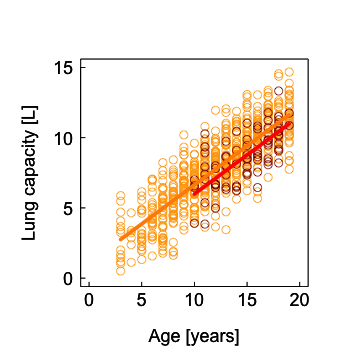
\includegraphics[width=0.5\textwidth]{lectures/day_3_LM_refresh_II/figures/unnamed-chunk-31-1.png}
   \end{tabular}
   &
   \begin{tabular}{l}
       \parbox{0.4\linewidth}{
         When predictors are correlated \textbf{and} both influence the response, multivariate regression prevents the \textbf{omitted variable bias}!
        }
   \end{tabular}
 \end{tabular}
\end{frame}

\begin{frame}
    \frametitle{}
    \textbf{BUT}, imagine $x_1$ fully correlates with $x_2$ so that e.g.: $x_2 = 2 * x_1$ Then:
    \begin{equation*}
        \begin{aligned}
        y = 5 + 2 * x_1 + 1 * x_2 \\
        \textit{or } y = 5 + 2 * x_2 \\
        \textit{or } y = 5 + 4 * x_1 \\
        \textit{ etc. ...}
        \end{aligned}
    \end{equation*}
    \vspace{0.5cm}
    
    The Log-Likelihood can be equally high for different combinations of the coefficients for $x_2$ and $x_2$\\
    \textbf{= bad estimates and high standard errors}
\end{frame}

\begin{frame}
  \frametitle{}
  \textbf{Correlated predictors make it difficult to estimate coefficients because of \textit{variance inflation}.}
  \\
  Remember the variance estimation for the linear coefficient:
  \begin{equation*}
      cov(\hat{\beta}_j) = \sigma(\textbf{X'X})^{-1}
  \end{equation*}

  This can be reformulated to:
  
  \begin{equation*}
    Var(\hat{\beta}_j) = \frac{1}{(1-R^2)} \cdot \frac{\sigma^2}{\sum_{i=1}^{n} (x_{ij} - \overline{x}_j)^2}
  \end{equation*}
  
  A small model variance $\sigma^2$ and a small $R^2$ lead to small variances of $\hat{\beta}$.
\end{frame}

\begin{frame}
    \frametitle{We have a dilemma...}
    \large{Too few correlated predictors distort results \textbf{(the omitted variable bias)}, but too many correlated predictors can, too \textbf{(variance inflation)}.}
\end{frame}

\begin{frame}
  \frametitle{Variance - Bias Trade-off}
  \textbf{The problem of minimizing two sources of errors.}
  
  \begin{itemize}
    \item Either high explained variance but low generality (\textit{overfitting the data}).
    \item Or low bias (high general insights) but lower fit to the specific data.
  \end{itemize}
  
  \begin{center}
    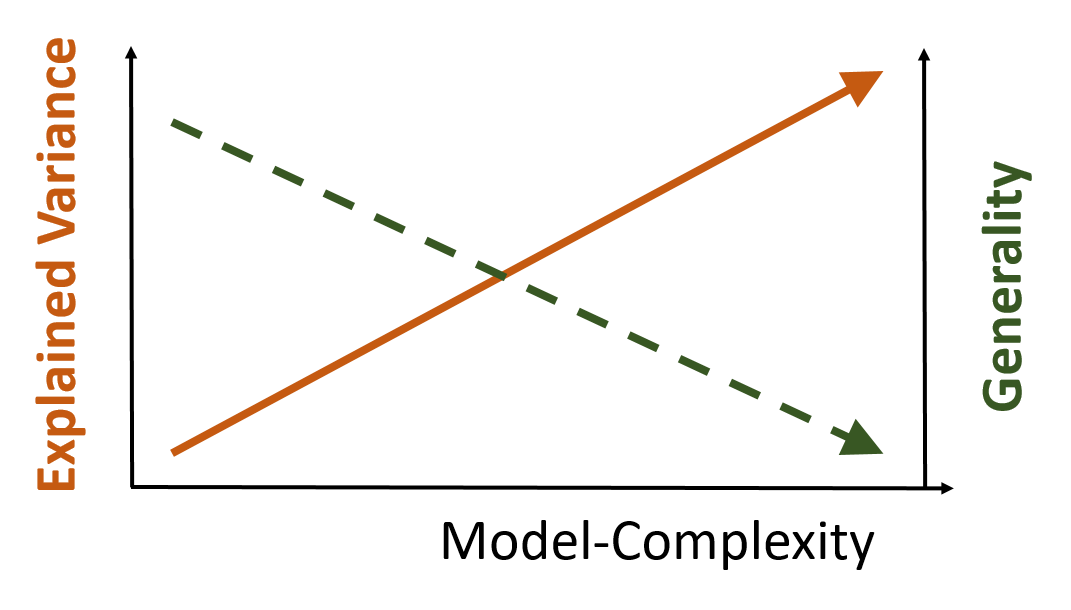
\includegraphics[width=0.9\textwidth]{figures/var-bias-tradeoff.png} 
  \end{center}
\end{frame}

\begin{frame}
  \frametitle{Overfitting}
  \textbf{Too many predictors can cause \textit{Overfitting}.}
  
  \begin{itemize}
    \item A model overfits the data when it re-draws the specifics of the dataset but doesn't deliver general/transferable insights.
  \end{itemize}
  
  \begin{center}
    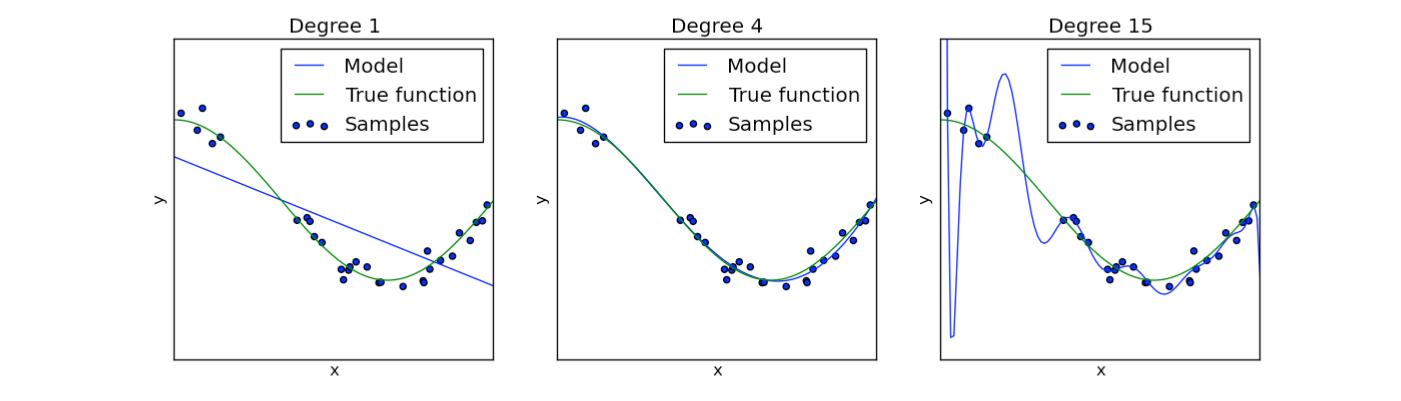
\includegraphics[width=1\textwidth]{figures/overfitting.png} 
  \end{center}
\end{frame}

\begin{frame}{}
  \begin{center}
    \huge\textbf{\textcolor{purple}{Interactions between predictors}}
  \end{center}
\end{frame}

\begin{frame}
  \frametitle{Linear Model Without Interaction}
  \textbf{Additive model}
  
  The two predictors are associated with the response independently of each other.
  
  \begin{equation*}
    y = \beta_0 + \beta_1 \cdot x_1 + \beta_2 \cdot x_2 + \epsilon
  \end{equation*}
\end{frame}

\begin{frame}
  \frametitle{Including an Interaction}
  \textbf{Multiplicative model}
  
  The effect of one predictor on the response depends on the values of another predictor:
  
  \begin{equation*}
    y = \beta_0 + \beta_1 \cdot x_1 + \beta_2 \cdot x_2 + \beta_3 \cdot (x_1 \times x_2) + \epsilon
  \end{equation*}
  
  There is now a third parameter $\beta_3$ for the interaction.
\end{frame}

\begin{frame}
  \frametitle{}
  Interaction between two categorical (binary) predictors.
  
  \begin{itemize}
    \item $x_1$: Coffee machine ($A$: French press or $B$: De'Longhi)
    \item $x_2$: Coffee type ($1$: Lavazza or $2$: Schwarzwild)
    \item Response: some proxy for taste
  \end{itemize}
  
  \begin{center}
    \includegraphics[width=0.6\textwidth]{lectures/day_3_LM_refresh_II/figures/unnamed-chunk-boxplot_interaction_image} 
  \end{center}
\end{frame}

\begin{frame}
  \frametitle{}
  Interaction between a categorical and a continuous predictor.
  
  \begin{itemize}
    \item $x_1$: Nutrient score (color code)
    \item $x_2$: Temperature
  \end{itemize}
  
  \begin{center}
    \includegraphics[width=0.6\textwidth]{lectures/day_3_LM_refresh_II/figures/unnamed-chunk-scatterplot_interaction_image} 
  \end{center}
\end{frame}

\begin{frame}
  \frametitle{Interaction Coefficients}
  What do the interaction coefficients tell us?
  
  \begin{equation*}
    y = \beta_0 + \beta_1 \cdot x_1 + \beta_2 \cdot x_2 + \beta_3 \cdot (x_1 \times x_2) + \epsilon
  \end{equation*}
\end{frame}

\begin{frame}
  \frametitle{Recapitulation Day 3}
  After today, you should know and understand:
  \begin{itemize}
    \item What the difference between \textbf{continuous} and \textbf{categorical} predictors is.
    \item How \textbf{multiple} predictors can be included in a statistical model.
    \item What an \textbf{interaction} between predictors is.
    \item What R functions to use.
  \end{itemize}
  
  \vspace{1cm}
  Today afternoon: practical exercises about \textbf{categorical} and \textbf{multiple predictors} and \textbf{interactions} in R.
\end{frame}

\end{document}
